\section{User Interface}
\subsection{Description}
When the sensor data has arrived at the remote PC, the data has to be read out. The data should be at least be output to a console. If possible due to time constraints, the data will be more visualised.
\subsubsection{CUI}
The CUI (Console User Interface) is the most basic way the data will be output. All the sensor data will be output to the control with corresponding label. The CUI will automatically be updated when new data arrives. 
\begin{figure}[H]
	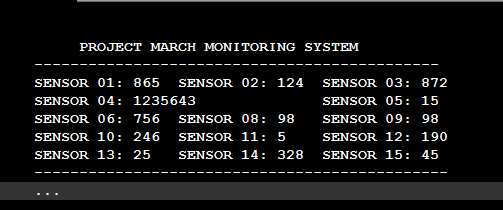
\includegraphics{MockupCUI}
	\caption{A mock-up with a possible look of the CUI} 
\end{figure} 
\subsubsection{GUI}
The GUI (Graphic User Interface) consists of two parts. One part shows a dashboard with the most important sensor data visualised. The other part is a concise list with all sensor data.  
\begin{figure}[H]
	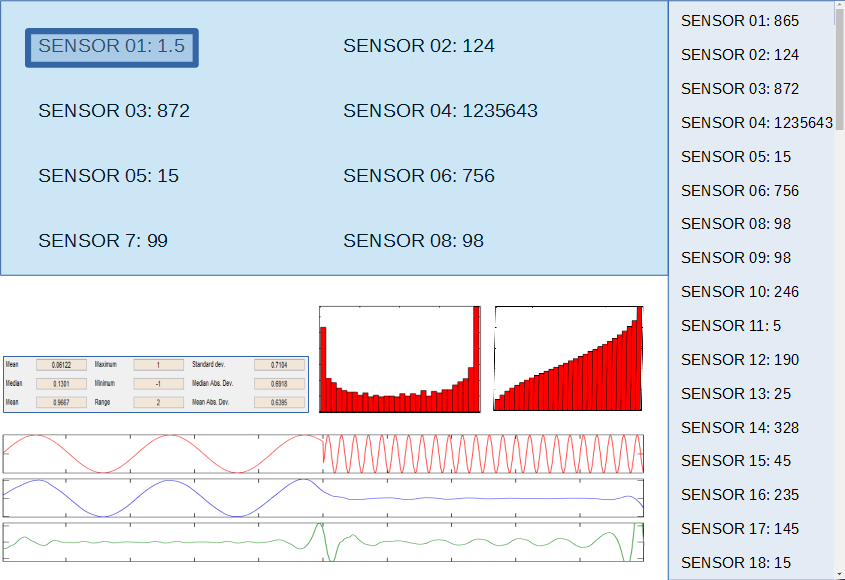
\includegraphics[width=500px]{MockupGUI}
	\caption{A mock-up with a possible look of the GUI} 
\end{figure} 
\subsection{Framework}
In order to choose a language, there are two important factors in this project which have to be taken in account. Firstly, the framework should have a rich support of visualising data. Secondly, the framework must be able to support 3D rendering. Keeping this in mind, the options of languages are narrowed down to C/C++, Java \& Python because these are known to have a rich selection of libraries which support 3D rendering and data visualisation. In addition, since SimuLink is a Matlab module, using Matlab as framework is also an option. \\
The requirements state that data visualisation has a higher priority than 3D-rendering. Because of this, it is not essential that the chosen framework has an extensive 3D-library. In the end, Matlab was chosen as preferred framework for the GUI for the following reasons:
\begin{itemize}
	\item The required data is sent through SimuLink, which is a module of Matlab. This means that the data does not need to be converted.
	\item Matlab has an extensive collection of data visualisation tools.
	\item Most other applications within Project MARCH also make use of Matlab. Therefore, using Matlab helps future integration and easier continuation.
\end{itemize}
In the event that it proves to be impossible or undesirable to connect wireless directly using Matlab, there are two alternatives to consider. The first one is to create a receiver which listens on the port and can convert the data to a format which is readable by Matlab. The other option is to create the GUI in HTML as a web-page and put a web-socket in the page to get the data. This implementation is very user friendly, as the only required software for the client is a web-browser. In addition, this makes it very easy for multiple people to use the monitoring system since the exoskeleton will broadcast over the wi-fi instead of sending the data directly to another client. By using this method, the options for the framework are limited to JavaScript and its libraries. In addition, running code in a browser tends to be less powerful than running the code in a stand-alone application. This results in a lower update frequency and fewer options for data visualising.

\subsection{3D-Rendering}
Because of the fact that the 3d-rendering has shifted to a lower priority, less effort has been expended in researching suitable frameworks for rendering. Still, a small list have been compiled of some rendering frameworks which are simple to use for each of the narrowed down languages.
\begin{itemize}
	\item C/C++: Ogre3D
	\item Java/Scala: Env3D
	\item Python: Panda3D
\end{itemize}
	